% A LaTeX (non-official) template for ENSI projects reports
% Copyright (C) 2025 ENSI


\documentclass[12pt,a4paper]{report}

% Encodage et langues
\usepackage[utf8]{inputenc}  % Encodage UTF-8 (obsolète mais utile pour pdflatex)
\usepackage[T1]{fontenc}     % Encodage des fontes
\usepackage[french]{babel}  % Langue principale du document
%\usepackage[english]{babel}  % Décommentez si vous écrivez en anglais

% Mise en page et marges
\usepackage{geometry}        % Configuration des marges
\geometry{a4paper, margin=2.5cm}

% Gestion des titres et en-têtes/pieds de page
\usepackage{titlesec}        % Personnalisation des titres
\titleformat{\chapter}[frame]{\normalfont\huge\bfseries}{\chaptername\ \thechapter}{20pt}{\Huge}
\usepackage{fancyhdr}        % Personnalisation des en-têtes et pieds de page
\pagestyle{fancy}
\renewcommand{\chaptermark}[1]{\markboth{#1}{#1}}
\fancyhead[R]{\thepage}
\fancyhead[L]{\chaptername\ \thechapter\ --\ \leftmark}

% Mathématiques
\usepackage{amsmath, amssymb, amsthm, bm}

% Algorithmes
\usepackage{algorithm}
\usepackage{algpseudocode}
%\usepackage{listofalgorithms} % Pour générer la liste des algorithmes

% Gestion des images et figures
\usepackage{graphicx}        % Inclusion d'images
\graphicspath{{images/}}     % Chemin par défaut des images
\usepackage{subfig}          % Sous-figures
\usepackage{float}           % Positionnement exact des figures

% Tableaux et mises en page avancées
\usepackage{array, multirow} 

% Gestion des références et bibliographies
\usepackage{hyperref}        % Liens cliquables dans le PDF
\usepackage[footnote]{acronym} % Acronymes en note de bas de page
\usepackage[resetlabels,labeled]{multibib} % Bibliographies multiples
\newcites{URL}{Netography}  % Bibliographie spécifique aux sources Internet
\newcites{URL}{Netographie}  % Bibliographie spécifique aux sources Internet
\usepackage{url}            % Formatage des URL

% Texte en arabe (pour pdflatex uniquement)
\usepackage{arabtex}         % Texte arabe
\usepackage{utf8}            % Assurer la compatibilité UTF-8

% Gestion des sous-fichiers
\usepackage{subfiles}

% Définition de tailles pour figures
\newlength\figureheight
\newlength\figurewidth
% si le rapport est écrit en français
\renewcommand{\listalgorithmname}{Liste des Algorithmes} % Mettre en commentaire en cas de rapport en anglais
% Insertition de fichier pdf
\usepackage{pdfpages}

\begin{document}

%%%%%%%%%%%%%%%%%%
%%% Page de garde %%%
%%%%%%%%%%%%%%%%%%

\subfile{pg-ENSI} 
%\subfile{pg-ENSI_ang} % if english report
\clearpage
%%%%%%%%%%%%%%%%%%%%%%%%%%%%%%%%%%%%%%%%%%%%%%%%%%%%%%%%%%
    %%% Remerciements, tables de matières, etc %%%
%%%%%%%%%%%%%%%%%%%%%%%%%%%%%%%%%%%%%%%%%%%%%%%%%%%%%%%%%%

%\frontmatter

\clearpage
\subfile{0-i-signature}
\clearpage
% Insérer le résumé

% Écrire votre résumé en trois langues dans le fichier Résumé.docx.
% Convertir Resume.docx en Resume.pdf.

% Ajouter le fichier dans main.tex :
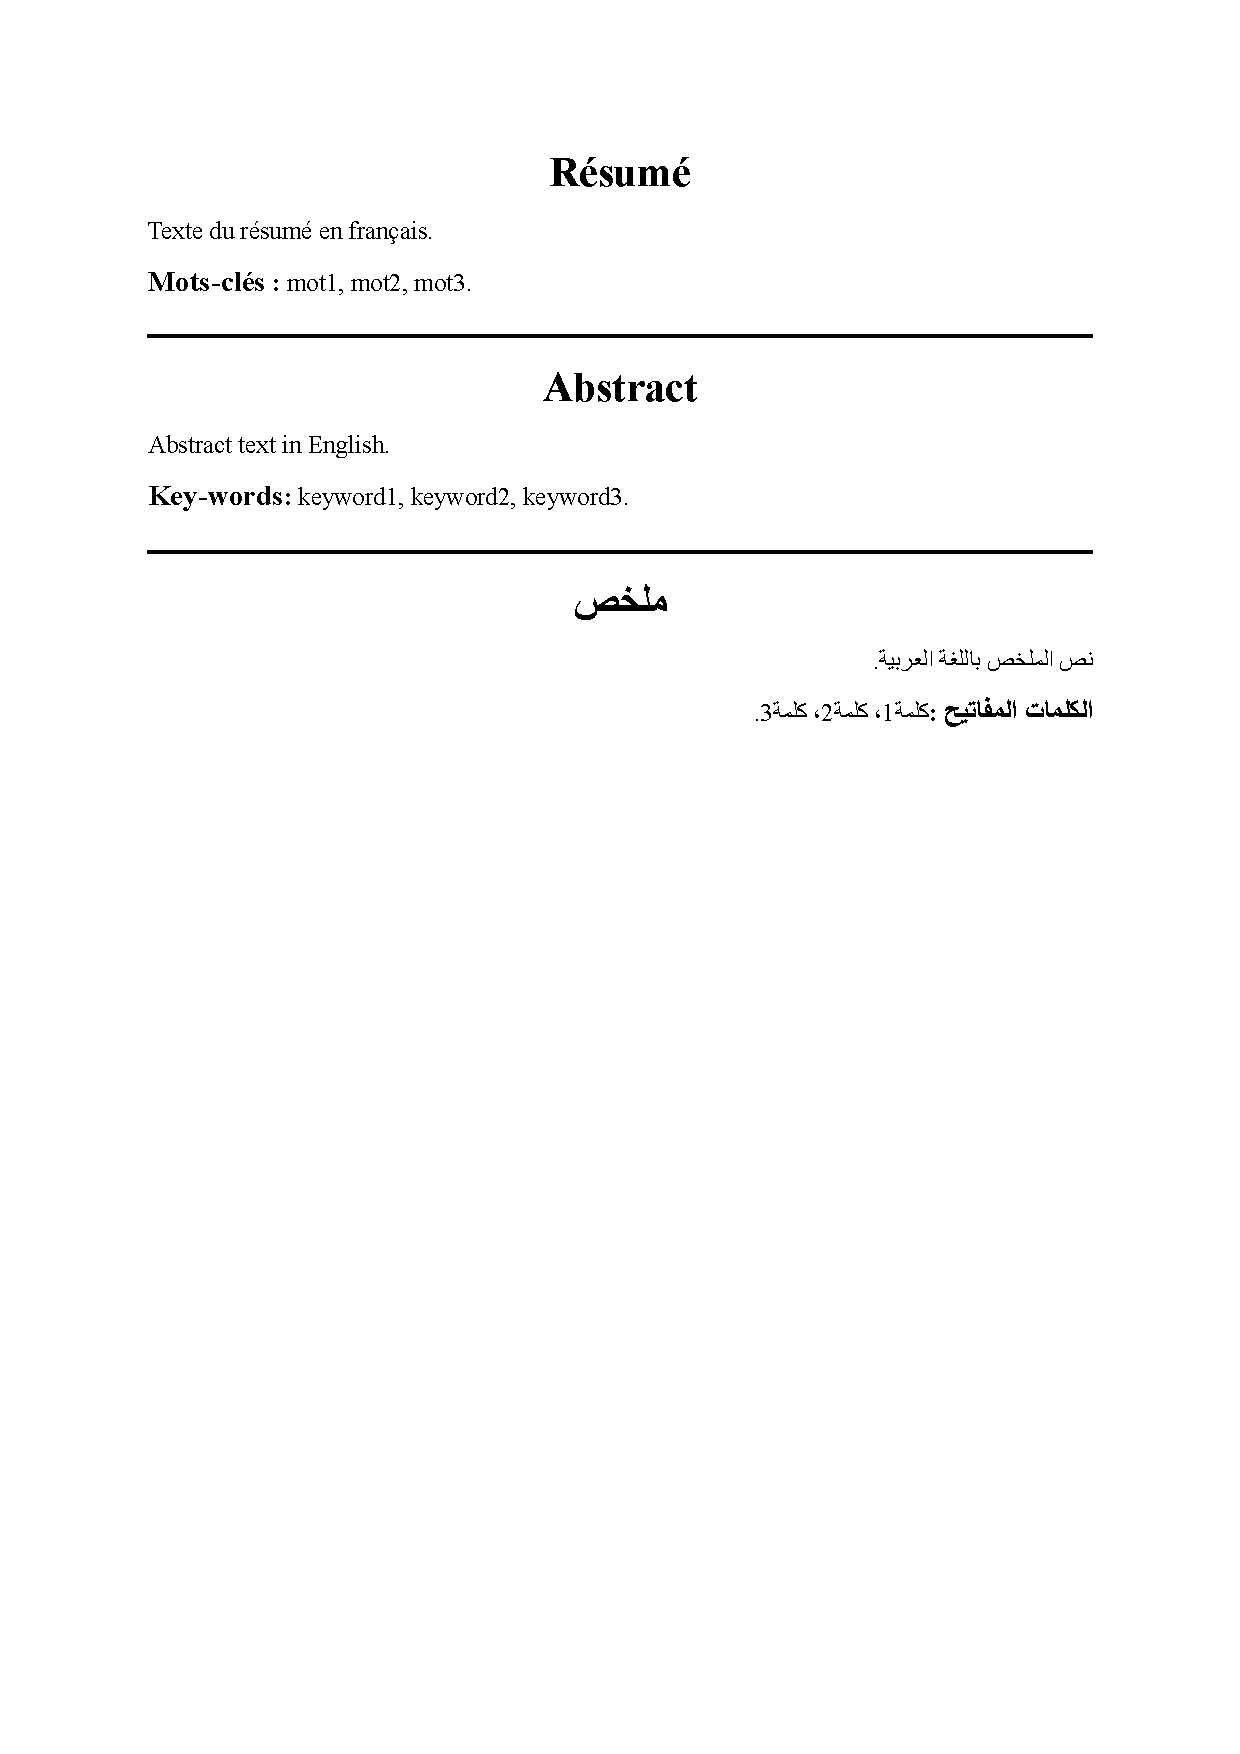
\includepdf[pages=-]{Resume.pdf}
\clearpage
\pagenumbering{roman}
\subfile{0-iii-Remerciements}
\clearpage
\tableofcontents
\clearpage
\listoffigures
\clearpage
\listoftables
\clearpage
\listofalgorithms
\clearpage
%\chapter*{Liste des acronymes}
\chapter*{List of acronyms}% if english report
\begin{acronym}[ACRO5] % Give the longest acronym here
\acro{ACRO1}{\emph{ACRONYME1}}
\acro{ACRO2}{\emph{ACRONYME2}}
\acro{ACRO3}{\emph{ACRONYME3}}
\acro{ACRO4}{\emph{ACRONYME4}}
\acro{ACRO5}{\emph{ACRONYME5}}
\end{acronym}

%%%%%%%%%%%%%%%%%%%%%%%%%%%%%%%%%%%%%%%%%%%%
%%% Corps du rapport et les références %%%
%%%%%%%%%%%%%%%%%%%%%%%%%%%%%%%%%%%%%%%%%%%%


\pagestyle{fancy}

\cleardoublepage
\pagenumbering{arabic}
\subfile{0-introduction}
\subfile{1-first-chapter}
\subfile{2-project-implementation}
\subfile{3-skills-development}
\subfile{2-conclusion}

% Annexes
\appendix
\subfile{3-annexes}


\renewcommand{\refname}{Bibliographie}
\bibliographystyle{plain}
\bibliography{references}\addcontentsline{toc}{chapter}{Bibliographie}
%\bibliography{references}\addcontentsline{toc}{chapter}{Bibliography}% if english report

\bibliographystyleURL{plain}
\bibliographyURL{urls}\addcontentsline{toc}{chapter}{Netographie}
%\bibliographyURL{urls}\addcontentsline{toc}{chapter}{Netography}% if english report

\end{document} 